        %%******************************************%%
        %%                                          %%
        %%        Modello di tesi di laurea         %%
        %%            di Andrea Giraldin            %%
        %%                                          %%
        %%             2 novembre 2012              %%
        %%                                          %%
        %%******************************************%%


% I seguenti commenti speciali impostano:
% 1. 
% 2. PDFLaTeX come motore di composizione;
% 3. tesi.tex come documento principale;
% 4. il controllo ortografico italiano per l'editor.

% !TEX encoding = UTF-8
% !TEX TS-program = pdflatex
% !TEX root = tesi.tex
% !TEX spellcheck = it-IT

% PDF/A filecontents
\RequirePackage{filecontents}
\begin{filecontents*}{\jobname.xmpdata}
  \Title{Analisi e sviluppo di una applicazione web per la schedulazione e rendicontazione delle attività aziendali interne}
  \Author{Riccardo Pavan}
  \Language{it-IT}
  \Subject{Questa tesi di laurea descrive il lavoro svolto e i risultati ottenuti durante il periodo di stage presso Wavelop Srls, con sede a Treviso. L'obiettivo del tirocinio era lo sviluppo di una applicazione web dedicata alla gestione delle attività aziendali interne, in particolare a mostrarle in formato sia tabellare che grafico, permettendo di filtrarle in vari modi. La tesi si propone inoltre di descrivere la metodologia di lavoro adottata e le tecnologie utilizzate per lo sviluppo della applicazione.}
  \Keywords{Applicazione web\sep Visualizzazione dati\sep React\sep Node.js \sep MongoDB}
\end{filecontents*}

\documentclass[10pt,                    % corpo del font principale
               a4paper,                 % carta A4
               twoside,                 % impagina per fronte-retro
               openright,               % inizio capitoli a destra
               english,                 
               italian,                 
               ]{book}    

%**************************************************************
% Importazione package
%************************************************************** 

\PassOptionsToPackage{dvipsnames}{xcolor} % colori PDF/A
\usepackage[table]{xcolor}
\usepackage{colorprofiles}
\usepackage{makecell}
\usepackage[a-2b,mathxmp]{pdfx}[2018/12/22]
                                        % configurazione PDF/A
                                        % validare in https://www.pdf-online.com/osa/validate.aspx

%\usepackage{amsmath,amssymb,amsthm}    % matematica

\usepackage[T1]{fontenc}                % codifica dei font:
                                        % NOTA BENE! richiede una distribuzione *completa* di LaTeX

\usepackage[utf8]{inputenc}             % codifica di input; anche [latin1] va bene
                                        % NOTA BENE! va accordata con le preferenze dell'editor

\usepackage[english, italian]{babel}    % per scrivere in italiano e in inglese;
                                        % l'ultima lingua (l'italiano) risulta predefinita

\usepackage{bookmark}                   % segnalibri

\usepackage{caption}                    % didascalie

\usepackage{chngpage,calc}              % centra il frontespizio

\usepackage{csquotes}                   % gestisce automaticamente i caratteri (")

\usepackage{emptypage}                  % pagine vuote senza testatina e piede di pagina

\usepackage{epigraph}			% per epigrafi

\usepackage{eurosym}                    % simbolo dell'euro

%\usepackage{indentfirst}               % rientra il primo paragrafo di ogni sezione

\usepackage{graphicx}                   % immagini

\usepackage{hyperref}                   % collegamenti ipertestuali

\usepackage[binding=5mm]{layaureo}      % margini ottimizzati per l'A4; rilegatura di 5 mm

\usepackage[]{listings}                   % codici

\usepackage{microtype}                  % microtipografia

\usepackage{mparhack,fixltx2e,relsize}  % finezze tipografiche

\usepackage{nameref}                    % visualizza nome dei riferimenti                                      
\usepackage[font=small]{quoting}        % citazioni

\usepackage{subfig}                     % sottofigure, sottotabelle

\usepackage[italian]{varioref}          % riferimenti completi della pagina

\usepackage{booktabs}                   % tabelle                                       
\usepackage{tabularx}                   % tabelle di larghezza prefissata                                    
\usepackage{longtable}                  % tabelle su più pagine                                        
\usepackage{ltxtable}                   % tabelle su più pagine e adattabili in larghezza

\usepackage[toc, acronym]{glossaries}   % glossario
                                        % per includerlo nel documento bisogna:
                                        % 1. compilare una prima volta tesi.tex;
                                        % 2. eseguire: makeindex -s tesi.ist -t tesi.glg -o tesi.gls tesi.glo
                                        % 3. eseguire: makeindex -s tesi.ist -t tesi.alg -o tesi.acr tesi.acn
                                        % 4. compilare due volte tesi.tex.

\usepackage[backend=biber,style=verbose-ibid,hyperref,backref]{biblatex}
                                        % eccellente pacchetto per la bibliografia; 
                                        % produce uno stile di citazione autore-anno; 
                                        % lo stile "numeric-comp" produce riferimenti numerici
                                        % per includerlo nel documento bisogna:
                                        % 1. compilare una prima volta tesi.tex;
                                        % 2. eseguire: biber tesi
                                        % 3. compilare ancora tesi.tex.

%**************************************************************
% file contenente le impostazioni della tesi
%**************************************************************

%**************************************************************
% Frontespizio
%**************************************************************

% Autore
\newcommand{\myName}{Riccardo Pavan}                                    
\newcommand{\myTitle}{Analisi e sviluppo di una applicazione web per la schedulazione e rendicontazione delle attività aziendali interne}

% Tipo di tesi                   
\newcommand{\myDegree}{Tesi di laurea}

% Università             
\newcommand{\myUni}{Università degli Studi di Padova}

% Facoltà       
\newcommand{\myFaculty}{Corso di Laurea in Informatica}

% Dipartimento
\newcommand{\myDepartment}{Dipartimento di Matematica "Tullio Levi-Civita"}

% Titolo del relatore
\newcommand{\profTitle}{Prof.}

% Relatore
\newcommand{\myProf}{Davide Bresolin}

% Luogo
\newcommand{\myLocation}{Padova}

% Anno accademico
\newcommand{\myAA}{2021-2022}

% Data discussione
\newcommand{\myTime}{Dicembre 2022}


%**************************************************************
% Impostazioni di impaginazione
% see: http://wwwcdf.pd.infn.it/AppuntiLinux/a2547.htm
%**************************************************************

\setlength{\parindent}{14pt}   % larghezza rientro della prima riga
\setlength{\parskip}{0pt}   % distanza tra i paragrafi


%**************************************************************
% Impostazioni di biblatex
%**************************************************************
\bibliography{bibliografia} % database di biblatex 

\defbibheading{bibliography} {
    \cleardoublepage
    \phantomsection 
    \addcontentsline{toc}{chapter}{\bibname}
    \chapter*{\bibname\markboth{\bibname}{\bibname}}
}

\setlength\bibitemsep{1.5\itemsep} % spazio tra entry

\DeclareBibliographyCategory{opere}
\DeclareBibliographyCategory{web}

\defbibheading{opere}{\section*{Riferimenti bibliografici}}
\defbibheading{web}{\section*{Siti Web consultati}}


%**************************************************************
% Impostazioni di caption
%**************************************************************
\captionsetup{
    tableposition=top,
    figureposition=bottom,
    font=small,
    format=hang,
    labelfont=bf
}


%**************************************************************
% Impostazioni di graphicx
%**************************************************************
\graphicspath{{immagini/}} % cartella dove sono riposte le immagini


%**************************************************************
% Impostazioni di hyperref
%**************************************************************
\hypersetup{
    %hyperfootnotes=false,
    %pdfpagelabels,
    %draft,	% = elimina tutti i link (utile per stampe in bianco e nero)
    colorlinks=true,
    pdfstartpage=1,
    pdfstartview=,
    % decommenta la riga seguente per avere link in nero (per esempio per la stampa in bianco e nero)
    %colorlinks=false, linktocpage=false, pdfborder={0 0 0}, pdfstartpage=1, pdfstartview=FitV,
    breaklinks=true,
    pdfpagemode=UseNone,
    pageanchor=true,
    pdfpagemode=UseOutlines,
    plainpages=false,
    bookmarksnumbered,
    bookmarksopen=true,
    bookmarksopenlevel=1,
    hypertexnames=true,
    pdfhighlight=/O,
    %nesting=true,
    %frenchlinks,
    urlcolor=webbrown,
    linkcolor=RoyalBlue,
    citecolor=webgreen,
    %pagecolor=RoyalBlue,
    urlcolor=Black, linkcolor=Black, citecolor=Black, %pagecolor=Black,
}

%**************************************************************
% Impostazioni di itemize
%**************************************************************
\renewcommand{\labelitemi}{$\ast$}

%\renewcommand{\labelitemi}{$\bullet$}
%\renewcommand{\labelitemii}{$\cdot$}
%\renewcommand{\labelitemiii}{$\diamond$}
%\renewcommand{\labelitemiv}{$\ast$}


%**************************************************************
% Impostazioni di listings
%**************************************************************
\lstset{
    language=[LaTeX]Tex,%C++,
    keywordstyle=\color{RoyalBlue}, %\bfseries,
    basicstyle=\small\ttfamily,
    %identifierstyle=\color{NavyBlue},
    commentstyle=\color{Green}\ttfamily,
    stringstyle=\rmfamily,
    numbers=none, %left,%
    numberstyle=\scriptsize, %\tiny
    stepnumber=5,
    numbersep=8pt,
    showstringspaces=false,
    breaklines=true,
    frameround=ftff,
    frame=single
} 


%**************************************************************
% Impostazioni di xcolor
%**************************************************************
\definecolor{webgreen}{rgb}{0,.5,0}
\definecolor{webbrown}{rgb}{.6,0,0}


%**************************************************************
% Altro
%**************************************************************

\newcommand{\omissis}{[\dots\negthinspace]} % produce [...]

% eccezioni all'algoritmo di sillabazione
\hyphenation
{
    ma-cro-istru-zio-ne
    gi-ral-din
}

\newcommand{\sectionname}{sezione}
\addto\captionsitalian{\renewcommand{\figurename}{Figura}
                       \renewcommand{\tablename}{Tabella}}

\newcommand{\glsfirstoccur}{\ap{{[g]}}}

\newcommand{\intro}[1]{\emph{\textsf{#1}}}

%**************************************************************
% Environment per ``rischi''
%**************************************************************
\newcounter{riskcounter}                % define a counter
\setcounter{riskcounter}{0}             % set the counter to some initial value

%%%% Parameters
% #1: Title
\newenvironment{risk}[1]{
    \refstepcounter{riskcounter}        % increment counter
    \par \noindent                      % start new paragraph
    \textbf{\arabic{riskcounter}. #1}   % display the title before the 
                                        % content of the environment is displayed 
}{
    \par\medskip
}

\newcommand{\riskname}{Rischio}

\newcommand{\riskdescription}[1]{\textbf{\\Descrizione:} #1.}

\newcommand{\risksolution}[1]{\textbf{\\Soluzione:} #1.}

%**************************************************************
% Environment per ``use case''
%**************************************************************
\newcounter{usecasecounter}             % define a counter
\setcounter{usecasecounter}{0}          % set the counter to some initial value

%%%% Parameters
% #1: ID
% #2: Nome
\newenvironment{usecase}[2]{
    \renewcommand{\theusecasecounter}{\usecasename #1}  % this is where the display of 
                                                        % the counter is overwritten/modified
    \refstepcounter{usecasecounter}             % increment counter
    \vspace{10pt}
    \par \noindent                              % start new paragraph
    {\large \textbf{\usecasename #1: #2}}       % display the title before the 
                                                % content of the environment is displayed 
    \medskip
}{
    \medskip
}

\newcommand{\usecasename}{UC}

\newcommand{\usecaseactors}[1]{\textbf{\\Attori Principali:} #1. \vspace{4pt}}
\newcommand{\usecasepre}[1]{\textbf{\\Precondizioni:} #1. \vspace{4pt}}
\newcommand{\usecasedesc}[1]{\textbf{\\Descrizione:} #1. \vspace{4pt}}
\newcommand{\usecasepost}[1]{\textbf{\\Postcondizioni:} #1. \vspace{4pt}}
\newcommand{\usecasealt}[1]{\textbf{\\Scenario Alternativo:} #1. \vspace{4pt}}

%**************************************************************
% Environment per ``namespace description''
%**************************************************************

\newenvironment{namespacedesc}{
    \vspace{10pt}
    \par \noindent                              % start new paragraph
    \begin{description} 
}{
    \end{description}
    \medskip
}

\newcommand{\classdesc}[2]{\item[\textbf{#1:}] #2}
                     % file con le impostazioni personali
\begin{document}
%**************************************************************
% Materiale iniziale
%**************************************************************
\frontmatter
% !TEX encoding = UTF-8
% !TEX TS-program = pdflatex
% !TEX root = ../tesi.tex

%**************************************************************
% Frontespizio 
%**************************************************************
\begin{titlepage}

\begin{center}

\begin{LARGE}
\textbf{\myUni}\\
\end{LARGE}

\vspace{10pt}

\begin{Large}
\textsc{\myDepartment}\\
\end{Large}

\vspace{10pt}

\begin{large}
\textsc{\myFaculty}\\
\end{large}

\vspace{30pt}
\begin{figure}[htbp]
\begin{center}

\includegraphics[height=6cm]{logo-unipd}
\end{center}
\end{figure}
\vspace{30pt} 

\begin{LARGE}
\begin{center}
\textbf{\myTitle}\\
\end{center}
\end{LARGE}

\vspace{10pt} 

\begin{large}
\textsl{\myDegree}\\
\end{large}

\vspace{40pt} 

\begin{large}
\begin{flushleft}
\textit{Relatore}\\ 
\vspace{5pt} 
\profTitle \myProf
\end{flushleft}

\vspace{-52pt} 

\begin{flushright}
\textit{Laureando}\\ 
\vspace{5pt} 
\myName
\end{flushright}
\end{large}

\vspace{40pt}

\line(1, 0){338} \\
\begin{normalsize}
\textsc{Anno Accademico \myAA}
\end{normalsize}

\end{center}
\end{titlepage} 
% !TEX encoding = UTF-8
% !TEX TS-program = pdflatex
% !TEX root = ../tesi.tex

%**************************************************************
% Colophon
%**************************************************************
\clearpage
\phantomsection
\thispagestyle{empty}

\hfill

\vfill

\noindent\myName: \textit{\myTitle,}
\myDegree,
\textcopyright\ \myTime.
% !TEX encoding = UTF-8
% !TEX TS-program = pdflatex
% !TEX root = ../tesi.tex

%**************************************************************
% Sommario
%**************************************************************
\cleardoublepage
\phantomsection
\pdfbookmark{Sommario}{Sommario}
\begingroup
\let\clearpage\relax
\let\cleardoublepage\relax
\let\cleardoublepage\relax

\chapter*{Sommario}

Il presente documento descrive il lavoro svolto durante il periodo di stage, della durata di circa trecento ore, dal laureando Pinco Pallino presso l'azienda Azienda S.p.A.
Gli obbiettivi da raggiungere erano molteplici.\\
In primo luogo era richiesto lo sviluppo di ...
In secondo luogo era richiesta l'implementazione di un ... 
Tale framework permette di registrare gli eventi di un controllore programmabile, quali segnali applicati 
Terzo ed ultimo obbiettivo era l'integrazione ...

%\vfill
%
%\selectlanguage{english}
%\pdfbookmark{Abstract}{Abstract}
%\chapter*{Abstract}
%
%\selectlanguage{italian}

\endgroup			

\vfill


% !TEX encoding = UTF-8
% !TEX TS-program = pdflatex
% !TEX root = ../tesi.tex

%**************************************************************
% Ringraziamenti
%**************************************************************
\cleardoublepage
\phantomsection
\pdfbookmark{Ringraziamenti}{ringraziamenti}

\begin{flushright}{
	\slshape    
	``Life is really simple, but we insist on making it complicated''} \\ 
	\medskip
    --- Confucius
\end{flushright}


\bigskip

\begingroup
\let\clearpage\relax
\let\cleardoublepage\relax
\let\cleardoublepage\relax

\chapter*{Ringraziamenti}

\noindent \textit{Innanzitutto, vorrei esprimere la mia gratitudine al Prof. NomeDelProfessore, relatore della mia tesi, per l'aiuto e il sostegno fornitomi durante la stesura del lavoro.}\\

\noindent \textit{Desidero ringraziare con affetto i miei genitori per il sostegno, il grande aiuto e per essermi stati vicini in ogni momento durante gli anni di studio.}\\

\noindent \textit{Ho desiderio di ringraziare poi i miei amici per tutti i bellissimi anni passati insieme e le mille avventure vissute.}\\
\bigskip

\noindent\textit{\myLocation, \myTime}
\hfill \myName

\endgroup


% !TEX encoding = UTF-8
% !TEX TS-program = pdflatex
% !TEX root = ../tesi.tex

%**************************************************************
% Indici
%**************************************************************
\cleardoublepage
\pdfbookmark{\contentsname}{tableofcontents}
\setcounter{tocdepth}{2}
{
    \hypersetup{linkcolor=black}
    \tableofcontents
}
%\markboth{\contentsname}{\contentsname} 
\clearpage

\begingroup 
    \let\clearpage\relax
    \let\cleardoublepage\relax
    \let\cleardoublepage\relax
    %*******************************************************
    % Elenco delle figure
    %*******************************************************    
    \phantomsection
    \pdfbookmark{\listfigurename}{lof}
    \listoffigures

    \vspace*{8ex}

    %*******************************************************
    % Elenco delle tabelle
    %*******************************************************
    \phantomsection
    \pdfbookmark{\listtablename}{lot}
    \listoftables
        
    \vspace*{8ex}
\endgroup

\cleardoublepage

\cleardoublepage

%**************************************************************
% Materiale principale
%**************************************************************
\mainmatter
\chapter{L'azienda}
\label{cap:azienda}

\section{Descrizione generale}

\begin{center}
	
\includegraphics[height = 4cm]{wavelop-logo.png}
\end{center}

\noindent Wavelop S.R.L.S. è una giovane azienda nata nel 2018 con sede a Treviso che si occupa di consulenza e di progetti web e mobile per piccole e medie imprese.\\
L'azienda conta circa 10 dipendenti e offre un ambiente lavorativo giovane e dinamico. Predilige inoltre lo smartworking e la flessibilità degli orari.\\
Dal 2020 propone progetti per studenti universitari che siano interessati in un tirocinio presso la loro azienda. 

(progetti anche per clienti reali, inserimento in un team di lavoro)

\section{Modello di svluppo}

Wavelop segue un modello di sviluppo \textit{agile} con metodologia \textit{scrum}. Di seguito le caratteristiche che contraddistinguono questo metodo di lavoro:

\begin{itemize}
  \item il lavoro viene diviso in archi temporali della durata di una settimana, denominati \textit{sprint};
  \item all'inizio di ogni \textit{sprint} si tiene lo \textit{sprint planning}, una riunione in cui si chiarisce quali obiettivi, espressi sotto forma di \textit{user stories}, si mira a portare a termine;
  \item alla fine di ogni \textit{sprint} si tiene invece lo \textit{sprint review}, una riunione in cui si discute cosa si è fatto durante lo \textit{sprint}, mostrando i risultati ottenuti, anche tramite brevi demo anche ai clienti;
  \item all'inizio di ogni giornata lavorativa si partecipa allo \textit{stand-up meeting}, una breve riunione della durata di circa 15 minuti, dove, a turno, ogni membro del team espone brevemente cosa ha fatto il giorno precedente e cosa intende fare oggi, oltre che mettere al corrente tutti di eventuali ostacoli incontrati nello sviluppo.
\end{itemize}

Adottare una metodologia di questo tipo permette una comunicazione costante fra i membri del team e i clienti che porta a un tracciamento chiaro e preciso dell'avanzamento del progetto e a una messa in luce immediata di eventuali incomprensioni, permettendo quindi delle correzioni tempestive, in accordo col cliente.
% !TEX encoding = UTF-8
% !TEX TS-program = pdflatex
% !TEX root = ../tesi.tex

%**************************************************************
\chapter{Descrizione dello stage}
\label{cap:descrizionestage}
%**************************************************************

\section{Il progetto}

L'azienda ha già iniziato a sviluppare un'applcazione web, denominata \emph{Timesheet}, desitinata a uso interno, al fine di rendicontare e pianificare le attività dei vari componenti dell'azienda. \\
In particolare è già implementata la funzionalità di inserire attività singole nel database. \\
Manca, invece, la possibilità di mostrare, filtrandole a seconda della volontà dell'utente, le varie attività memorizzate, ottenendo quindi dati utili come la quantità di ore dedicate a un cliente in un determinato arco di tempo. \\
Queste funzionalità dovranno essere raggruppate nella sezione \emph{Reports} dell'applicazione. \\
Lo scopo finale del progetto è quindi quello di completare la sezione \emph{Reports}, sia per quanto riguarda la componente di frontend che per quella di backend.

\section{Requisiti}
\label{sec:requisiti}
Nel piano di lavoro sono stati redatti requisiti specifici che dovranno essere soddisfatti nel periodo di stage. Essi sono categorizzati in base alla importanza che ricoprono:


\paragraph{Obbligatori} Requisiti ad alta priorità, la cui importanza è primaria per la riuscita del progetto:

\begin{itemize}
  \item apprendimento delle tecnologie di sviluppo come React e Node.js e per il versionamento del progetto come git;
  \item gestione filtri avanzati di ricerca delle attività;
  \item visualizzazione a tabella delle attività filtrate;
  \item generazione file CSV delle attività filtrate.
\end{itemize}

\paragraph{Desiderabili} Requisiti a media priorità, non nececssari per il completamento dello stage ma che comunque, se soddisfatti, contribuiscono notevolmente alla buona riuscita del progetto: 

\begin{itemize}
  \item generazione file PDF delle attività filtrate;
  \item visualizzazione attività tramite grafico;
  \item salvataggio preset filtri per ricerche future.
\end{itemize} 

\paragraph{Facoltativi} Requisiti a bassa priorità, portano un valore aggiunto allo stage:

\begin{itemize}
  \item visualizzazione widget laterale con statistiche relative all'utente;
  \item gestione responsive della piattaforma.
\end{itemize}

\section{Pianificazione}

Lo stage ha avuto luogo nel periodo di tempo dal 25 Luglio 2022 al 16 Settembre 2022, per un totale di 312 ore.
Sono state inoltre definite delle attività specifiche per ogni settimana di stage, rappresentate di seguito:

\paragraph{Prima settimana - Dal 25 al 29 Luglio}

\begin{itemize}
  \item discussione requisiti relativi al sistema da sviluppare con le persone coinvolte nel progetto;
  \item introduzione alla cultira aziendale;
  \item formazione sulle tecnologie adottate;
  \item prendere confidenza con la struttura già esistente e assegnazione degli strumenti necessari;
  \item analisi dei requisiti.
\end{itemize}

\noindent\textbf{Seconda settimana - Dall'1 al 5 Agosto}

\begin{itemize}
  \item analisi dei requisiti;
  \item progetazione architetturale.
\end{itemize}

\noindent\textbf{Terza settimana - Dall'8 al 13 Agosto}

\begin{itemize}
  \item progettazione architetturale;
  \item analisi e definizione user stories per lo sprint successivo.
\end{itemize}

\noindent\textbf{Dalla quarta alla ottava settimana - Dal 16 Agosto al 16 Settembre}

\begin{itemize}
  \item sviluppo delle user stories assegnate;
  \item sprint review con il referente e le altre persone coinvolte nel progetto;
  \item analisi e definizione user stories per lo sprint successivo.
\end{itemize}

\noindent Inoltre, nell'ultima settimana, è previsto un collaudo finale di ciò che è stato fatto.

\section{Tecnologie utilizzate}

È stato utilizzato lo stack tecnologico tipicamente scelto dall'azienda, composto da: \emph{Ract}, \emph{Node.js} e \emph{MongoDB}, di seguito descritte nel dettaglio, una per una.

\subsection{React}

React\footcite{site:react} è una libreria Javascript open-source component-based per creare interfacce utente mantenuta da \emph{Meta}. Adotta l'utilizzo di una sintassi che estende il linguaggio Javascript: il \emph{Javascript Synstax Extension} (JSX), che rende semplice e intuitivo creare i componenti che formano la pagina.\\
\begin{code}[frame=tb,title={Esempio di utlizzo di codice JSX}]
1  const name = 'Riccardo Pavan';
2
3  const ShowName = () => {
4    return (
5      <div>Mi chiamo {name}</div>
6    );
7  };

\end{code}

Un'altra particolarità di React sono gli \emph{hooks}, particolari funzioni che permettono di "agganciarsi" a varie funzionalità di \emph{lifecycle} che React offre senza dovere usare classi.

\subsection{Node.Js}

Node.Js\footcite{site:node.js} è un \emph{runtime environment} open-source basato su Javascript.\\
La sua architettura orientata agli eventi permette alle operazioni di input/output di essere asincrone ed è consona soprattutto per applicazioni scalabili e che necessitano di un grande \emph{throughput} .\\
L'utilizzo di Node.Js permette di utilizzare Javascript anche lato server, permettendo quindi di usarlo come unico linguaggio nello sviluppo di un'applicazione web, dando vita al paradigma detto \emph{Javascript everywhere}.\\

\subsection{MongoDB}

MongoDB\footcite{site:mongo} è un \emph{database manaegement system} open-source non relazionale, orientato ai documenti, questi ultimi in formato BSON, simile a JSON.\\
La struttura non relazionale permette una maggiore libertà nello strutturare il database, utile quando si ha a che fare con molti dati molto diversi fra loro e che tendono a cambiare nel tempo.             
% !TEX encoding = UTF-8
% !TEX TS-program = pdflatex
% !TEX root = ../tesi.tex

%**************************************************************
\chapter{Sprint 1}
\label{cap:sprint1}
%**************************************************************

Descrizione del primo sprint.             
% !TEX encoding = UTF-8
% !TEX TS-program = pdflatex
% !TEX root = ../tesi.tex

%**************************************************************
\chapter{Sprint 2}
\label{cap:sprint2}
%**************************************************************

Durante il secondo sprint ho redatto la versione conclusiva del documento relativo alle user stories, approvato poi dal mio relatore esterno.

\noindent Ogni user story del documento presenta i seguenti elementi:
\begin{itemize}
  \item nome della useer story;
  \item un numero intero positivo che indica il "peso" in termini temporali che ci si aspetta che la user story abbia. Questi numeri seguono l'andamento della serie di Fibonacci e sono stati utli per allocare meglio le varie user stories all'interno degli sprint; 
  \item breve descrizione di ciò che si deve ottenere una volta conclusa la user story, dal punto di vista dell'utente;
  \item elenco di task, suddivisi tra frontend e backend, che dicono in modo più speccifico e tecnico cosa fare per concludere la user story;
\end{itemize}

\noindent All'inizio di ogni capitolo relativo a uno sprint indicherò le user stories su cui andrò a lavorare.

Ho inoltre creato dei diagrammi UML dei casi d'uso. (Li metto qua?)

Per concludere la settimana ho lavorato a dei piccoli bugfix e features, anche per familiarizzare con la web app e i pattern utilizzati.
In particolare ho: 
\begin{itemize}
  \item sistemato un problema con la immagine nella pagina di login, che non si rimpiccioliva nel caso la finestra facesse lo stesso;
  \item fatto sì che, nella pagina utente, nel caso quest'ultimo non la avesse inserita, venissero mostate le iniziali dell'utente invece che nulla;
  \item implementato una finestra di dialogo che semplicemente chiede di confermare o annullare un'azione.
\end{itemize}

Seppure i primi due problemi fossero molto semplici e risolvibili principalmente con del codice CSS, creare la finestra di dialogo mi è stato utile sia a familiarizzare con React, che non avevo mai utilizzato, ma anche a capire meglio come fosse strutturata la applicazione.
             
% !TEX encoding = UTF-8
% !TEX TS-program = pdflatex
% !TEX root = ../tesi.tex

%**************************************************************
\chapter{Sprint 3}
\label{cap:sprint3}
%**************************************************************
Descrizione del terzo sprint.             
% !TEX encoding = UTF-8
% !TEX TS-program = pdflatex
% !TEX root = ../tesi.tex

%**************************************************************
\section{Sprint 4}
\label{sec:sprint4}
%**************************************************************

\subsection{User stories assegnate}
\paragraph{Filtri utente, cliente, progetto e task (rispettivamente 5, 2, 2 e 2)}\mbox{} \\[\baselineskip]
\noindent Come utente autenticato che si trova nella sezione “Reports”, voglio poter scegliere uno o più utenti, clienti, progetti o task, anche contemporaneamente, e visualizzare le ore lavorative spese dal'utente o dedicate al cliente/progetto/task.\\

\noindent Tasks:

\begin{itemize}
  \item Implementare il componente dei filtri;
  \begin{itemize}
    \item implementare il componente principale;
    \item implementare lo stile per i filtri;
  \end{itemize}
  \item Implementare la logica di query nel backend per i filtri.
\end{itemize}

\subsection{Filtri utente, cliente, progetto e task}
\noindent A ciò che ho già fatto, è richiesto di aggiungere una toolbar, posizionata sopra la tabella, che permetta all'utente, tramite dei menù a tendina, di filtrare i dati che vengono mostrati, in particolare utenti, clienti, progetti e task. \\
Innanzitutto ho creato il component principale \texttt{ReportFilter} contenente la toolbar e i vari filtri. \\
Per creare elementi grafici come input, select, button ho utilizzato una librera grafica React già utilizzata nel resto della applicazione: MUI\footcite{site:mui}. In questo modo, oltre a mantenere una consistenza di stile con il rest della app, è risultato più facile interagire con questi elementi grafici (come tenere traccia di quali elementi sono selezionati nei select).\\
Successivamente, erano necessarie delle nuove richieste al backend per ottenere le liste di tutti gli utenti, clienti, progetti e task da mostrare nei rispettivi filtri. I vari endpoint erano già presenti, non ho quindi dovuto ancora toccare il backend per le richieste.\\
Avendo tutti i dati necessari, è stato sufficiente renderli disponibili al component principale \texttt{Reports} in modo da poterli usare nella richiesta per i dati già implementata. In particolare ho aggiunto i seguenti queryparams:
\begin{itemize}
  \item \texttt{users}: un array contenente gli utenti selezionati nei filtri;
  \item \texttt{clients}: un array contenente i clienti selezionati nei filtri;
  \item \texttt{projects}: un array contenente i progetti selezionati nei filtri;
  \item \texttt{tasks}: un array contenente i task selezionati nei filtri.
\end{itemize}
Ho modificato il backend di conseguenza, in modo che la query già implementata ottenesse solo le attività con, ad esempio, il campo \texttt{task} uguale a uno degli elementi presenti nell'array \texttt{tasks}. Con MongoDB questa è un'operazione piuttosto semplice in quanto basta utilizzare la keyword \texttt{\$match} che permette appunto di ottenere documenti che rispettano una condizione, come mostrato nell'esempio di codice \ref{code:mongo}.

\begin{code}[frame=tb, label={code:mongo}, caption={Esempio di filtro task lato backend con MongoDB}]\\
1  {
2    $match: tasks
3    ? { task: { $in: tasks } }
4    : { task: { $exists: true } },
5  },
\end{code}\\\\

\noindent In questo caso, se l'utente ha selezionato almeno un task, verrà eseguita la linea 3 del codice ottenendo solo i documenti con il campo \texttt{task} che compare in \texttt{tasks}, altrimenti verranno ottenuti tutti i documenti (linea 4).

\subsection{Sprint review}
La sprint review si è conclusa in modo positivo, senza particolari correzioni necessarie.
Anche i tempi sono stati rispettati.\\
Nella figura \ref{fig:report_filters} sono visibili i filtri realizzati, posizionati sopra la tabella.

\begin{figure}[H]
	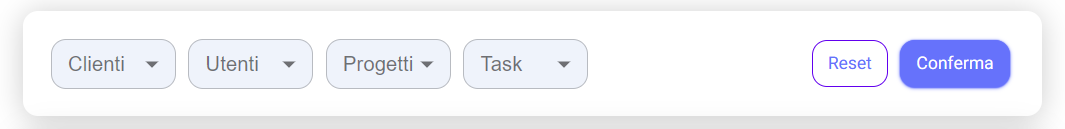
\includegraphics[width = \textwidth]{immagini/reports filters.png}
	\caption{Filtri della tabella}
	\label{fig:report_filters}
\end{figure}             
% !TEX encoding = UTF-8
% !TEX TS-program = pdflatex
% !TEX root = ../tesi.tex

%**************************************************************
\chapter{Sprint 5}
\label{cap:sprint 5}
%**************************************************************

\section{User stories assegnate}
\paragraph{Filtro temporale (8)}\mbox{} \\[\baselineskip]
Come utente autenticato che si trova nella sezione “Reports”, voglio poter filtrare i dati visualizzati in modo che coprano solo un determinato lasso di tempo. In particolare voglio poter visualizzare i dati:
\begin{itemize}
  \item del giorno corrente;
  \item della settimana corrente;
  \item del mese corrente; 
  \item dell'anno corrente.
\end{itemize}
O, in alternativa, impostare un arco temporale personalizzato, con date di inizio e fine a piacere.\\

\noindent Tasks:
\begin{itemize}
  \item ricerca su librerie che offrano elementi datepicker consoni ai requisiti;
  \item implementare il componente del filtro temmporale;
  \begin{itemize}
    \item implementare il componente principale;
    \item implementare lo stile per il filtro;
  \end{itemize}
  \item aggiungere le opzioni per selezionare giorno/settimana/mese/anno corrente e arco temporale personalizzato;
  \item aggiornare la logica di query lato backend.
\end{itemize} 

\section{Filtro temporale}
Con il team abbiamo concluso che la soluzione migliore per soddisfare questo requisito fosse l'aggiunta di un semplice bottone che, cliccato, espande un calendario dove l'utente può slezionare la data di inizio e di fine dell'arco temporale per cui vuole filtrare i dati. Inoltre, a fianco al calendario, devono essere presenti delle opzioni per impostare rapidamente gli archi di tempo predefiniti. \\
Per semplificare le cose ho fatto una breve ricerca su delle librerie che offrissero dei datepicker adatti, finendo col scegliere \texttt{react-date-range}\footcite{site:rdr}. Questa scelta è dovuta principalmente che già di suo permette di soddisfare tutte le problematiche del requisito, eccetto quella di espandere il calendario da un bottone, che comunque è risolvibile in modo piuttosto semplice. È inoltre molto intuitiva e semplice da utlizzare ed è piacevole esteticamente.\\
Per quanto riguarda il lato backend non ho dovuto fare niente poichè avevo già integrato i parametri \texttt{from} e \texttt{to} nella query al databse, sapendo che sarebbero serviti.\\\\
Infine, ho aggiunto un bottone per confermare i vari filtri per limitare il numero di richieste al backend. In questo modo verrà fatta una sola richiesta una volta che l'utente ha scelto tutti i filtri, invece che una dopo la selezione di ogni filtro.

\section{Sprint review}
La sprint review si è conclusa in modo positivo, senza particolari correzioni necessarie. Anche i tempi sono stati rispettati.             
% !TEX encoding = UTF-8
% !TEX TS-program = pdflatex
% !TEX root = ../tesi.tex

%**************************************************************
\section{Sprint 6}
\label{sec:sprint6}
%**************************************************************

%**************************************************************
\subsection{User stories assegnate}
\paragraph{Raggruppamento dati (11)}\mbox{} \\[\baselineskip]
Come utente autenticato che si trova nella sezione “Reports”, voglio poter raggruppare i dati visualizzati per utente, cliente, progetto, task e data, con un massimo di 3 livelli di profondità.\\
Ad esempio, raggruppando per utente, la tabella mostrerà due colonne:
\begin{itemize}
  \item \texttt{Utente}, con i nomi di ogni utente;
  \item \texttt{Ore}, con la somma delle ore delle attività di ogni utente.
\end{itemize}
Se poi voglio aggiungere un secondo livello di profondità al raggruppamento, ad esempio per cliente, la tabella mostrerà sempre la colonna \texttt{Utente}, ma questa volta, sotto a ogni nome, saranno presenti delle ulteriori righe con i nomi dei vari clienti per cui l'utente ha svolto attività, con relative somme di ore.\\

\noindent Tasks:
\begin{itemize}
  \item implementare la funzionalità di raggruppamento;
  \item aggiungere la possibilità di raggruppamenti multipli;
  \item aggiungere una nuova sezione filtri dedicata ai raggruppamenti.
\end{itemize}

\paragraph{Esportazione report in formato CSV (3)}\mbox{} \\[\baselineskip]
Come utente autenticato che si trova nella sezione “Reports”, voglio poter esportare il report correntemente mostrato in un file CSV. 
Esso dovrà contenere tutti i dati mostrati nella tabella (anche eventuali dati presenti nelle pagine non correntemente mostrate).\\

\noindent Tasks:
\begin{itemize}
  \item aggiungere opzione per eseportare la tabella in formato CSV;
  \item aggiungere logica per la generazione del file CSV lato backend.
\end{itemize}


\subsection{Raggruppamento dati}
La prima cosa che ho fatto è stata la parte di frontend, aggiungendo 3 menù a tendina, uno per ogni livello di raggruppamento, da cui scegliere il campo da raggruppare. Il secondo e terzo menù sono inizialmente nascosti e compaiono solo quando rispettivamente il primo e secondo raggruppamento sono stati scelti.\\
Lato frontend ho aggiornato la richiesta principale al backend aggiungendo 3 parametri: \texttt{groupOne}, \texttt{groupTwo} e \texttt{groupThree}. Essi sono stringhe che di default assumono il valore \texttt{none} ma, nel caso sia selezionato un raggruppamento da parte dell'utente, assumono il nome di quel raggruppamento, ad esempio \texttt{project}.\\
Ho inoltre creato un altro component per le righe ``raggruppate'', in modo da ottenere una struttura tale che, se l'utente ha scelto due raggruppamenti, vengano inizialmente mostrate le righe del primo raggruppamento, potendo visualizzare quelle del secondo cliccando sulla rispettiva riga, come mostrato nella figura \ref{fig:report_groupedtable}.\\\\
\begin{figure}[H]
	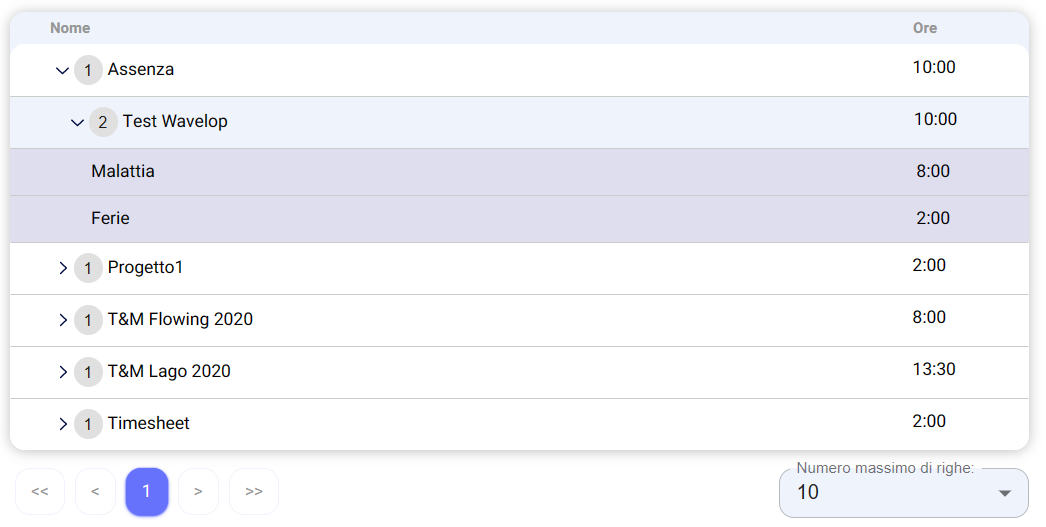
\includegraphics[width = \textwidth]{immagini/reports table groupings.png}
	\caption{Tabella che mostra dati raggruppati}
	\label{fig:report_groupedtable}
\end{figure}
Lato backend ho semplicemente aggiornato la query già presente in modo che potesse raggruppare i dati ottenuti, se richiesto. In questo caso i dati vengono ritornati con la seguente struttura:
\begin{itemize}
  \item \texttt{groupOne}
  \item \texttt{groupOneCount}
  \item \texttt{total}
\end{itemize}
Dove \texttt{groupOneCount} e \texttt{total} sono interi che rappresentano rispettivamente quanti elementi contiene il primo raggruppamento e la somma delle ore delle attività al suo interno.
\texttt{groupOne} è invece un array contenenti oggetti con la seguente struttura:
\begin{itemize}
  \item \texttt{name}: stringa contenente il nome della attività;
  \item \texttt{hours}: numero che rappresenta le ore dedicate all'attività;
  \item \texttt{groupTwo}: array contenente oggetti uguali a \texttt{groupOne}, eccetto relativi al secondo raggruppamento, più un campo \texttt{groupThree}.
\end{itemize}

\subsection{Esportazione report in formato CSV}
L'esportazione in formato CSV è risultata abbastanza rapida in quanto comportava solo ottenere i contenuti singoli dei campi richiesti dal frontend e porre tra di loro il carattere di separazione ``\texttt{,}''.\\
L'unica cosa a cui prestare attenzione è la eventuale presenza di virgole o virgolette nei campi che possano interferire col processo di separare i campi.
Per risolvere il problema basta circondare ogni campo tra virgolette.\\
Poi, tramite la funzione \texttt{join()}, ho unito tutti i campi di una riga ponendo fra loro il carattere \texttt{,} e separato le righe con il carattere di a capo \texttt{\textbackslash n}.\\
Lato frontend ho poi aggiunto un bottone che permette di scaricare il file CSV così creato.

\subsection{Sprint review}
La sprint review si è conclusa in modo positivo, ma è emerso un piccolo bug nella selezione dei raggruppamenti: selezionando primo, secondo e terzo raggruppamento e poi togliendo il secondo o il primo, il terzo raggruppamento rimaneva selezionato. La sistemazione di questo bug è rimasta assegnata per lo sprint 7.             
% !TEX encoding = UTF-8
% !TEX TS-program = pdflatex
% !TEX root = ../tesi.tex

%**************************************************************
\section{Sprint 7}
\label{sec:sprint7}
%**************************************************************

%**************************************************************
\subsection{User stories assegnate}

\paragraph{Esportazione report in formato PDF (8)}\mbox{} \\[\baselineskip]
Come utente autenticato che si trova nella sezione “Reports”, voglio poter esportare il report correntemente mostrato in un file PDF.
Esso dovrà contenere la tabella e il grafico mostrati nel report.\\

\noindent Tasks:
\begin{itemize}
  \item aggiungere opzione per eseportare la tabella in formato PDF;
  \item aggiungere logica per la generazione del file PDF lato backend.
\end{itemize}

\paragraph{Inclusione/esclusione colonne (3)}\mbox{} \\[\baselineskip]
Come utente autenticato che si trova nella sezione “Reports” e che sta esportando il proprio report, voglio poter selezionare quali colonne includere e quali no nel file PDF/CSV generato.\\

\noindent Tasks:
\begin{itemize}
  \item Aggiungere un modale dopo avere selezionato il tipo di file da generare che permetta di scegliere quali colonne escludere;
  \item Aggiungere logica per riflettere le scelte fatte nel file generato.
\end{itemize}

\subsection{Esportazione report in formato PDF}
Per la creazione di file PDF mi è stato consigliato l'utilizzo di due librerie: puppeteer\footcite{site:puppeteer} e Handlebars.js\footcite{site:handlebars}.\\
La prima permette di utilizzare una versione \textit{headless} (senza interfaccia utente) di un browser (in questo caso Chrome), la seconda, invece, mette a disposizione un linguaggio di templating HTML. L'idea è quindi di creare un template riutilizzabile per i report tramite Handlebars.js, per poi generarne un PDF tramite puppeteer, che verrà esportato.\\
Ho quindi creato il template tramite Handlebars.js che è risultato molto comodo e semplice grazie alle funzioni che la libreria mette a disposizione.

\begin{code}[frame=tb, label={code:handlebars}, caption={Esempio di utilizzo di Handlebars.js}]\\
1 {{#each people}}
2   <span>{{this.firstName}}</span> 
3   {{#if this.lastName}}
4     <span>{{this.lastName}}</span>
5   {{/if}}
6   <br>
7 {{/each}} 
\end{code}\\\\

\noindent L'esempio di codice \ref{code:handlebars} mostrato genererà, per ogni elemento presente in \texttt{people}, due tag \texttt{span} contenenti rispettivamente il valore della corrente iterazione di \texttt{people.firstName} e \texttt{people.lastName}, ma il secondo verrà generato solo se il campo \texttt{lastName} effettivamente esiste.\\
Una volta creato il template bisogna compilarlo tramite la funzione \texttt{compile()} di Handlebars.js per permettere a puppeteer di generare il relativo file PDF.

\begin{code}[frame=tb, label={code:puppeteer}, caption={Esempio di utilizzo di puppeteer per la creazione di file PDF}]\\
1   const template = Handlebars.compile(htmlTemplate);
2   const html = template(data);  
3   /*data contiene i dati che voglio mostrare nel report*/
4   const browser = await puppeteer.launch();
5   const page = await browser.newPage();
6 
7   await page.setContent(html, { waitUntil: "domcontentloaded" });
8 
9   const pdf = await page.pdf({
10     /*Opzioni di stile*/
11  });
12  await browser.close();
13  return pdf.toString("base64");
\end{code}\\\\

\noindent Nell'esempio di codice \ref{code:puppeteer} si può vedere come il browser headless venga lanciato (riga 4), venga creata una nuova pagina (riga 5), ne venga impostato il contenuto con l'HTML generato (riga 7) e ne venga generato il PDF (riga 9).\\
Una volta generato il PDF, esso viene mandato al client per poi essere scaricato.

\subsection{Inclusione/esclusione colonne}
Per questa user story la gran parte del lavoro è stata fatta nel frontend: ho fatto in modo che, una volta selezionato che si vuole esportare il file come CSV/PDF si aprisse una modale in cui l'utente può selezionare quali colonne includere o escludere, tramite delle spunte, e poi ho aggiornato la chiamata al backend in modo che mandasse anche queste scelte.\\
Nel backend è stato sufficiente rendere condizionale la creazione di ogni colonna di dati.

\subsection{Sprint review}
La sprint review si è conclusa in modo positivo, con solo dei miglioramenti estetici da fare ai documenti PDF creati per il prossimo sprint. Anche la correzione fatta al bug sorto durante la sprint review precedente è stata soddisfacente. 
% !TEX encoding = UTF-8
% !TEX TS-program = pdflatex
% !TEX root = ../tesi.tex

%**************************************************************
\chapter{Sprint 8}
\label{cap:sprint8}
%**************************************************************

%**************************************************************
Descrizione dell'ottavo sprint.
% !TEX encoding = UTF-8
% !TEX TS-program = pdflatex
% !TEX root = ../tesi.tex

%**************************************************************
\chapter{Conclusioni}
\label{cap:conclusioni}
%**************************************************************

%**************************************************************
\section{Il risultato finale}
Al termine di queste otto settimane ho portato a termine una sezione di una web app capabile di mostare all'utente dati relativi alle attività aziendali in formato sia tabellare che grafico e di esportarli.\\
Questi dati sono inoltre organizzabili in molti modi tramite le opzioni di filtro e di raggruppamento.\\\\
La figura \ref{fig:report_full} riporta una visione di insieme delle funzionalità sviluppate.\\
Partendo dall'alto, troviamo un bottone che di norma indica l'intervallo temporale correntemente selezionato, mentre cliccandoci sopra fa apparire il datepicker tramite il quale è possibile cambiarlo. Immediatamente sotto c'è la sezione filtri in cui è possibile selezionare quali clienti, utenti, progetti o task si voglia includere nei risultati. Sono presenti inoltre due pulsanti con la funzione rispettivamente di resettare i filtri allo stato di default o di confermarli.\\
Continuando verso il basso ci sono i raggruppamenti i cui secondo e terzo livello compaiono solo quando si è scelto il primo (figura \ref{fig:report_filters}. Sulla destra è inoltre presente un pulsante ``Esporta'' che permette di scegliere in che formato esportare i dati correntemente visualizzati.\\
Successivamente, dopo una riga dedicata a isualizzare le ore totali, c'è il grafico, seguito a sua volta dalla tabella. Entrambi questi elementi si aggiornano ad ogni cambiamento dei dati, anche se l'utente decide di raggrupparli. In particolare il grafico mostrerà sull'asse delle ascisse solo il primo raggruppamento, mentre la tabella assumerà la forma esposta in figura \ref{fig:report_groupedtable}.\\
Infine, il footer della tabella permette, con i tasti sulla sinistra di navigare le varie pagine della tabella, in caso ce ne fossero multiple, e, con il menù a tendina a destra, di scegliere quante righe per pagina impostare.
\clearpage
\begin{figure}[H]
	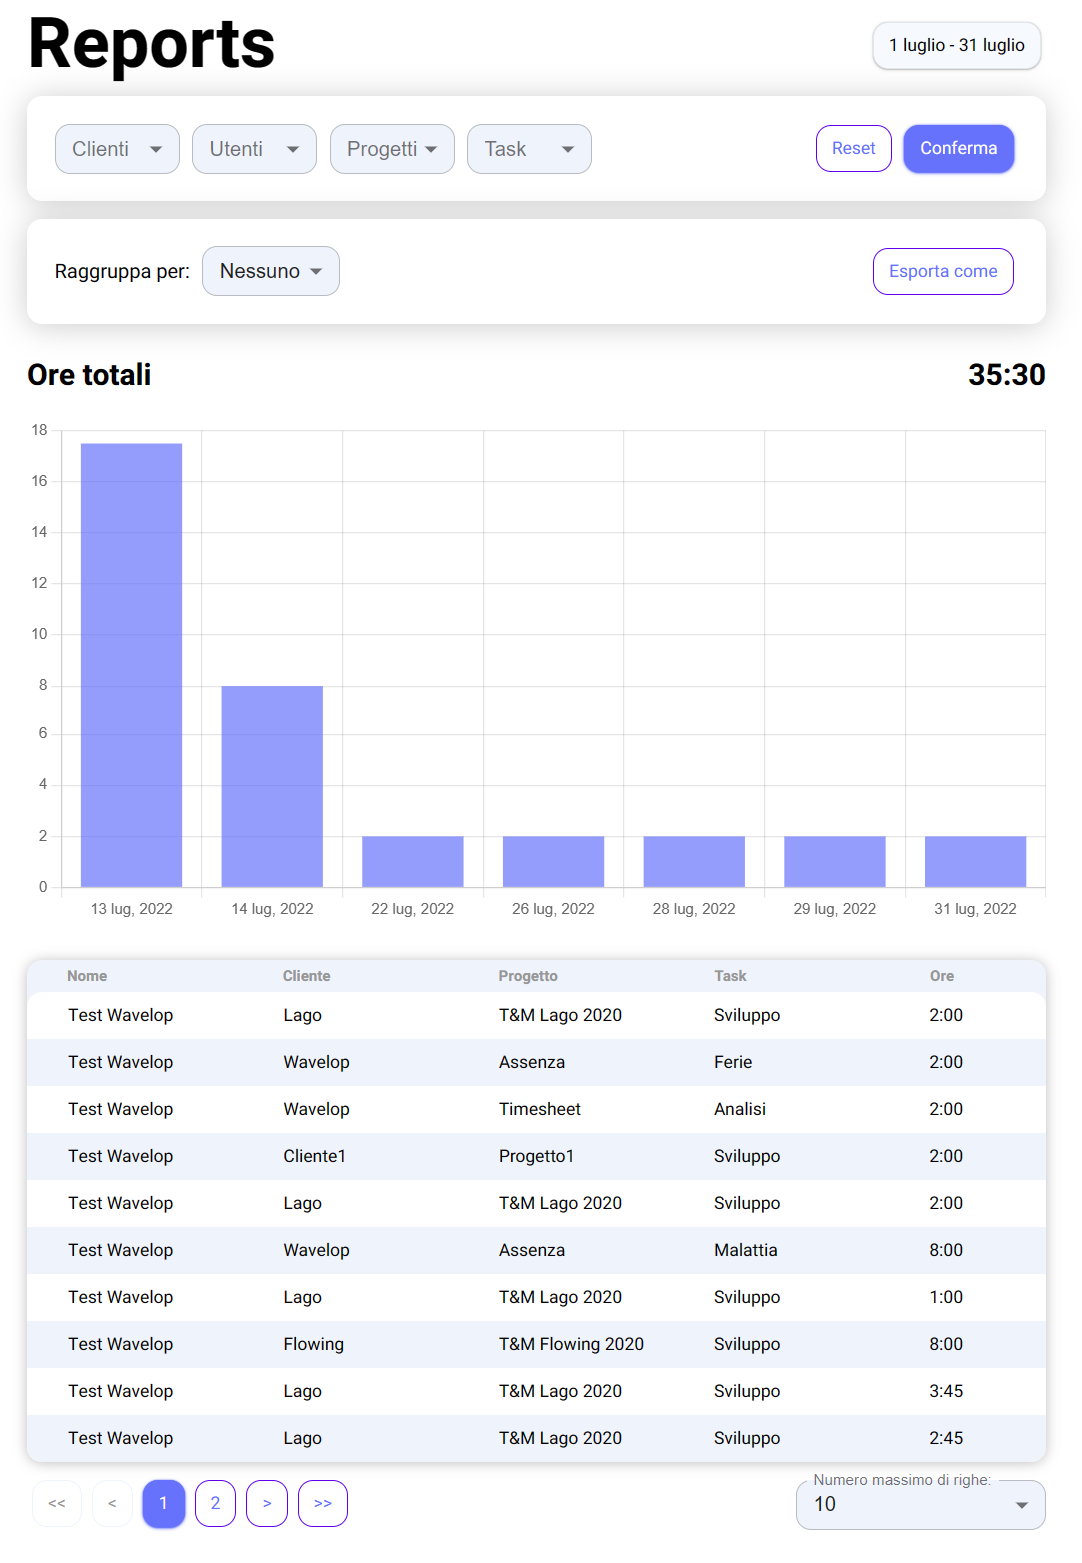
\includegraphics[width = \textwidth]{immagini/full reports.png}
	\caption{L'intera sezione Reports}
	\label{fig:report_full}
\end{figure}


\section{Soddisfazione dei requisiti}
La tabella seguente riporta lo stato di completamento dei requisiti elencati in \S\ref{sec:requisiti}.

\begin{table}[h]
	\centering
  \rowcolors{2}{gray!25}{white}
	\begin{tabularx}{\textwidth}{X|c|c}
    \rowcolor{white}
    \textbf{Requisito} & \textbf{Importanza} & \textbf{Stato} \\
    \hline
    \makecell[l]{Apprendimento delle tecnologie di sviluppo\\come React e Node.js e per il versionamento\\del progetto come git} & Obbligatorio & Rispettato \\
    \makecell[l]{Gestione filtri avanzati di ricerca delle attività} & Obbligatorio & Rispettato \\
    \makecell[l]{Visualizzazione a tabella delle attività filtrate} & Obbligatorio & Rispettato \\
    \makecell[l]{Generazione file CSV delle attività filtrate} & Obbligatorio & Rispettato \\
    \makecell[l]{Generazione file PDF delle attività filtrate} & Desiderabile & Rispettato \\
    \makecell[l]{Visualizzazione attività tramite grafico} & Desiderabile & Rispettato \\
    \makecell[l]{Salvataggio preset filtri per ricerche future} & Desiderabile & Non Rispettato \\
    \makecell[l]{Visualizzazione widget laterale con statistiche\\ relative all'utente} & Facoltativo & Non Rispettato \\
    \makecell[l]{Gestione responsive della piattaforma} & Facoltativo & \makecell{Parzialmente\\ rispettato} \\
	\end{tabularx}
	\vspace{5pt}
	\caption{Tabella dello stato di completamento dei requisiti}
	\label{tab:raggiungimento-obiettivi}
\end{table}

\noindent Seppure tutti i requisiti obbligatori sono stati tutti rispettati, ciò non è vero per alcuni desiderabili e facoltativi. Tale mancanza è principalmente dovuta al fatto che, durante lo stage, sono sorti altri requisiti che hanno avuto la precedenza su quelli non fatti (in particolare l'inclusione e l'esclusione delle colonne e il raggruppamento dati) e alla fine sono rimasti incompiuti. Ho inoltre segnato la gestione responsive della piattaforma come parzialmente rispettato poichè, andando avanti col progetto, ho gestito il responsive dei componenti che ho implementato, ma non c'è stato tempo di fare lo stesso per quelli rimanenti. 
\section{Valutazioni personali}
Questa esperienza di stage è stata un'ottima opportunità per mettere in pratica ciò che ho appreso durante il mio percorso di laurea.
In particolare da questa esperienza mi sono rimasti più di tutti questi insegnamenti:
\begin{itemize}
  \item il lavorare in un ambiente aziendale, seguendo  e rispettando dinamiche e metodologie ben definite e come influiscano positivamente sul lavoro;
  \item ho consolidato e arricchito le mie conoscenze sullo sviluppo di applicazioni web;
  \item ho imparato a utilizzare tecnologie che non avevo mai toccato prima d'ora e pratiche che avevo poco approfondito;
  \item ho imparato l'importanza della comunicazione e del confronto con i colleghi per collaborare alla risoluzione di un problema o al raggiungimento di un obiettivo, ma, allo stesso tempo, l'importanza di consultare la documentazione ufficiale per superare un ostacolo all'apparenza invalicabile.
\end{itemize}

\noindent Infine, voglio anche dire che questa è stata un'esperienza non solo utile ma anche piacevole, e che sono contento di finire il mio percorso universitario con questa opportunità.

%**************************************************************
% Materiale finale
%**************************************************************
\backmatter

\end{document}
